\section{Capacitors and Capacitance}

\begin{frame}{Introduction to Capacitors}
    \textbf{Capacitor}: generally two surfaces that \textbf{store charge}, with non-conductive material between plates.\\[5pt]
    \begin{tabular}{m{0.4\textwidth} m{0.5\textwidth}}
        & \multirow{3}{*}{
            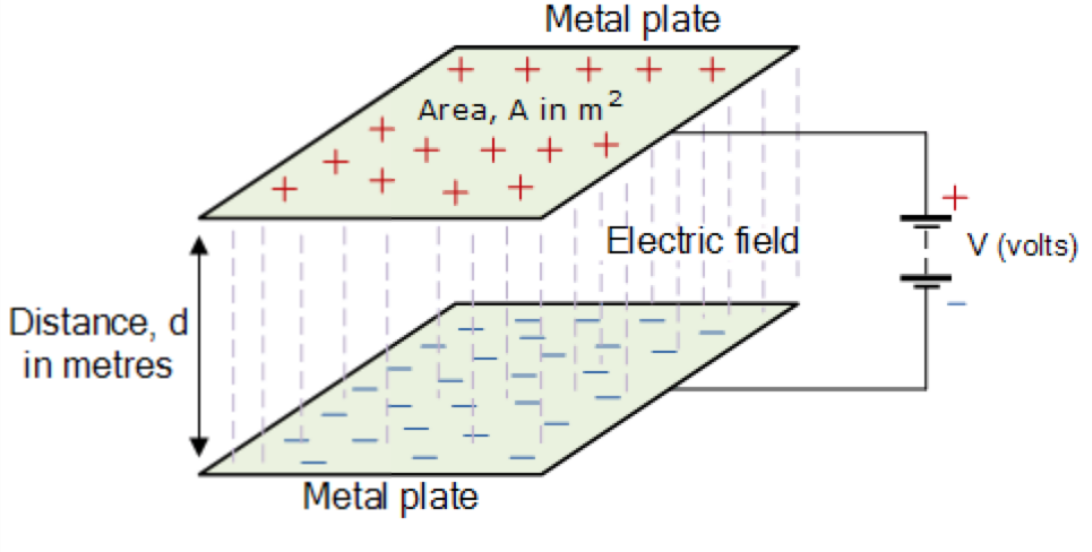
\includegraphics[width=0.5\textwidth]{images/capacitor.png}
        } \\
        $CV = Q$ \\
        $C = \epsilon A/d$ & \\[8pt]
    \end{tabular}
    \begin{itemize}
        \item $C$: capacitance
        \item $A$: area of capacitor (one plate)
        \item $d$: distance between plates
        \item $\epsilon$: “permittivity”, a constant depending on the material in the space between the two plates
    \end{itemize}
\end{frame}

\begin{frame}{Circuit model of a capacitor}
    \begin{tabular}{m{0.75\textwidth} m{0.15\textwidth}}
        Unit is the \textbf{Farad} (F) $\rightarrow$ Coulombs per volt ($C/V$) & \multirow{5}{*}{
            \begin{circuitikz}
                \draw (0, 2) to[C] (0, 0);
            \end{circuitikz}
        } \\[10pt]
        $C = Q/V$ & \\
        capacitance = charge/voltage ($F = C/V$) & \\[10pt]
        $E = \frac{1}{2} QV = \frac{1}{2} CV^2$ & \\
        \multicolumn{2}{c}{energy = 1/2 * capacitance * voltage squared ($J=C/V \cdot V^2 = CV$)}
    \end{tabular}
\end{frame}

\begin{frame}{Sanity Check: Parallel Plate Capacitor}
    \begin{align*}
        C = \epsilon \frac{A}{d}
    \end{align*}
    What is the \textbf{capacitance} of pair of parallel plates when 
    \begin{itemize}
        \item $A \to 0$?
        \item $A \to \infty$?
        \item $d \to 0$?
        \item $d \to \infty$? \\[10pt]
    \end{itemize}
    \textit{Does this make sense intuitively?}
\end{frame}

\begin{frame}{Sanity Check: Parallel Plate Capacitor [Solution]}
    \begin{align*}
        C = \epsilon \frac{A}{d}
    \end{align*}
    What is the \textbf{capacitance} of pair of parallel plates when 
    \begin{itemize}
        \item $A \to 0$? \textcolor{blue}{$C \to 0$}
        \item $A \to \infty$? \textcolor{blue}{$C \to \infty$}
        \item $d \to 0$? \textcolor{blue}{$C \to \infty$}
        \item $d \to \infty$? \textcolor{blue}{$C \to 0$}\\[10pt]
    \end{itemize}
    \textit{Does this make sense intuitively?} \\
    \textcolor{blue}{
        Yes, since as the area of the capacitor increases, the capacitor can hold more charge and vice versa. As the distance between the plates decreases, the charges escape to the other plate more easily.
    }
\end{frame}

\begin{frame}{Capacitors in Parallel}
    We know that the two capacitors must be at the \textbf{same voltage} but \textit{not necessarily have the same charge}. So: \\[10pt]
    \begin{tabular}{m{0.7\textwidth} m{0.2\textwidth}}
        $C_{eq} = Q/V$ & \multirow{4}{*}{
            \begin{circuitikz}[scale=0.7, transform shape]
                \draw (1, 3.75) to[short, -*] (1, 3)
                (0, 3) to[short] (2, 3)
                (0, 3) to[C=$C_1$] (0, 1)
                (2, 3) to[C=$C_2$] (2, 1)
                (0, 1) to[short] (2, 1)
                (1, 1) to[short, *-] (1, 0.25);
            \end{circuitikz}
        } \\
        $C_{eq} = (Q_1 + Q_2)/V$ & \\
        $C_{eq} = Q_1/V + Q_2/V$ & \\
        $C_{eq} = C_1 + C_2$ & \\
    \end{tabular}
\end{frame}

\begin{frame}{Capacitors in Parallel}
    \LARGE{
        TLDR: Just add them \\[5pt]
        $C_{eq} = \sum_n C_n$
    }
\end{frame}

\begin{frame}{Capacitors in Series}
    We know that both $C_1$ and $C_2$ have the \textbf{same charge} $Q$ stored in them since the \textit{current going through each of the capacitors must leave through the other}. On the other hand, the voltages \textbf{sum to the total voltage}. \\[10pt]
    \begin{tabular}{m{0.6\textwidth} m{0.3\textwidth}}
        Knowing this: & \multirow{4}{*}{
            \begin{circuitikz}[scale=0.7, transform shape]
                \draw (0, 2) to[V=$V$] (0, 0)
                (0, 2) to[C=$C_1$] (2, 2)
                (2, 2) to[C=$C_2$] (4, 2)
                (4, 2) to[short] (4, 0)
                (0, 0) to[short] (4, 0);
            \end{circuitikz}
        } \\
        $1/C_{eq} = (V_1 + V_2)/Q$ & \\
        $V_1/Q + V_2/Q$ & \\
        $1/C_{eq} = 1/C_1 + 1/C_2$ & \\
    \end{tabular}
\end{frame}

\begin{frame}{Capacitors in Series}
    \LARGE{
        TLDR: \\[5pt]
        $1/C_{eq} = \sum_n 1/C_n$
    }
\end{frame}

\begin{frame}{Equivalent Capacitance: Steps to Solve}
    \begin{itemize}
        \item \textbf{Decide} what \textbf{two nodes} you’re finding your capacitance over. \\
        \begin{itemize}
            \item Normally, it will be the capacitance between the \textit{terminals of a voltage or current source, or between two open terminals}.
        \end{itemize}
        \item \textbf{Break the problem down}: which capacitors are in \textbf{parallel}? Which capacitors are in \textbf{series}?
        \item \textbf{Use these equivalent capacitance equations} to simplify capacitances one “group” at a time until you are left with a single capacitance.
    \end{itemize}
    \textit{Note: Capacitor equations are exactly opposite of resistor equations!}
\end{frame}

\begin{frame}{Practice: Equivalent Capacitance}
    Find the \textbf{total capacitance} in this circuit.
    \begin{center}
        \begin{circuitikz}[scale=0.8, transform shape]
            \draw (5, 0) to[V=$V$] (0, 0)
            (0, 3) to[short] (0, 0)
            (0, 3) to[short] (0.5, 3)
            (0.5, 3.75) to[short] (0.5, 2.25)
            (0.5, 3.75) to[C=$C_1$] (2.5, 3.75)
            (0.5, 2.25) to[C=$C_1$] (2.5, 2.25)
            (2.5, 3.75) to[short] (2.5, 2.25)
            (2.5, 3) to[short] (3, 3)
            (3, 3) to[C=$C_3$] (5, 3)
            (5, 3) to[short] (5, 0);
        \end{circuitikz}
    \end{center}
\end{frame}

\begin{frame}{Practice: Equivalent Capacitance [Solution]}
    Find the \textbf{total capacitance} in this circuit. \\[5pt]
    \color{blue}
    \begin{tabular}{m{0.55\textwidth} m{0.35\textwidth}}
        The parallel portion becomes:  &
        \multirow{5}{*}{
            \color{black}
            \begin{circuitikz}[scale=0.55, transform shape]
                \draw (5, 0) to[V=$V$] (0, 0)
                (0, 3) to[short] (0, 0)
                (0, 3) to[short] (0.5, 3)
                (0.5, 3.75) to[short] (0.5, 2.25)
                (0.5, 3.75) to[C=$C_1$] (2.5, 3.75)
                (0.5, 2.25) to[C=$C_1$] (2.5, 2.25)
                (2.5, 3.75) to[short] (2.5, 2.25)
                (2.5, 3) to[short] (3, 3)
                (3, 3) to[C=$C_3$] (5, 3)
                (5, 3) to[short] (5, 0);
            \end{circuitikz}
        } \\
        $C_{par} = C_1 + C_2$ & \\[5pt]
        Then we use our series equation: \\
        $1/C_{eq} = 1/C_{par} + 1/C_3 = \frac{C_{par} + C_3}{C_{par} C_3}$ & \\[5pt]
        $C_{eq} = \frac{C_{par}C_3}{C_{par} + C_3} = \frac{C_1 C_3 + C_2 + C_3}{C_1 + C_2 + C_3}$ & \\
    \end{tabular}
\end{frame}

\begin{frame}{Charging a Capacitor}
    \begin{itemize}
        \item When a capacitor is supplied with current, it \textbf{charges up}.
        \item $V = Q/C$, so the voltage \textit{increases with time}.
        \item When the capacitor \textbf{discharges}, it \textit{loses charge and (therefore) voltage}. \\[5pt]
    \end{itemize}
    \underline{Working with charges over time}:
    \begin{itemize}
        \item Charge on capacitor after $t$ seconds (constant current): $I \cdot t$.
        \item $Q_{final} = C(V_{final} - V_{init})$
        \item $I = C dV/dt = C \Delta V / \Delta t$
        \item $C = I \Delta t / \Delta V$
        \item $Q_{final} = C \Delta V = I \Delta t = I(T_{final} = t_{init})$
    \end{itemize}
    \textit{Note: we'll be working with discrete time in 16A.}
\end{frame}